\documentclass[12pt,a4paper]{article}
\usepackage[utf8]{inputenc}
\usepackage{amsmath}
\usepackage{amsfonts}
\usepackage{amssymb}
\usepackage{makeidx}
\usepackage{graphicx}
\usepackage[left=2cm,right=2cm,top=2cm,bottom=2cm]{geometry}

\begin{document}
\title{\textbf{Sistemas electronicos de interfaz\\EV 1.3. Circuitos de control de voltaje y corriente con tiristores\\Practica 3}}
\author{Oscar Cruz Cervantes 18311797\\Ing. Mecatronica\\Grado 4B}
\date{30 de octubre del 2019}
\maketitle
\begin{figure}[h!]
\centering

\includegraphics[width=10cm]{UPCDLZMDG5783-logo.png} 
\end{figure}
\newpage

\section{Introducciòn}
En esta practica aprenderemos a utilizar 

\section{Objetivo}
Lograr hacer que el foco incandesente cambiara su intensidad modulando la misma con un potenciometro.

\section{Materiales}
Protoboard\\Resistencia de 1K\\Potenciometro de 500K\\Cables de protoboard\\Diac\\Triac\\Foco incandesente con clavija y base\\Laptop (Simulador a elegir)

\section{Desarrollo}
\textbf{1-} Como primera instancia de la practica, se procedera a simular el circuito para asi tener mas claro lo que se tiene que hacer y asi lograr ver errores antes de llegar a quemar alguno de nuestros componentes, el circuito en cuestiòn es el siguiente.
\begin{figure}[h!]
\centering
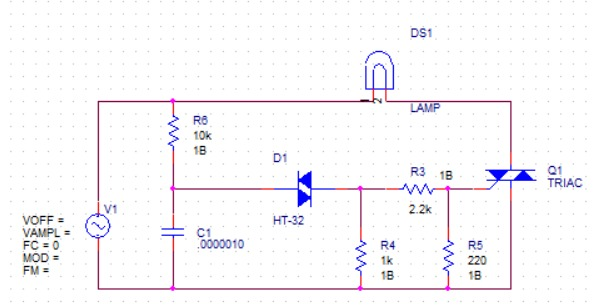
\includegraphics[scale=1]{01.jpeg}
\end{figure}

\textbf{2-} Una vez simulado se puede proceder a armarlo algo mas confiados ya que se vio anteriormente como es que puede llegar a reaccionar el circuito, claro en esta parte depende mas de como es que se le conecte asi que hacerlo con cuidado, en caso de duda preguntar a algun compañero o directamente con el asesor.\\

\textbf{3-} Una vez ya armado y funcionando, se debera de colocar marcas en el potenciometro para asi tener mas claro en que momento de la perilla la luz de nuestro foco comienza a obtener intensidad y cuando se le ve mas tenue, en este caso solo obtuvimos tres medidas, baja, media y alta. En algunos de los casos de los demas compañeros llegaron a obtener hasta 4 resultados diferentes.

\section{Conclusiòn}
Al final de la practica notamos distintas cosas, por ejemplo en el potenciometro que teniamos y cualquiera que conectaramos parecia que hacia un pequeño corto, pero no era asi del todo ya que esto se debia a el material por el cual estaba compuesto el potenciometro que era grafito, pero aun asi el resultado final de la practica fue positivo.
Tambien se descubrio que la forma de variar la intensidad variaba dependiendo que tipo de capacitor que le colocaras a tu circuito.\\
\textbf{-Oscar Cruz Cervantes}    

\end{document}